\documentclass[12pt]{article}
\usepackage[margin=1in]{geometry}
\usepackage[T1]{fontenc}
\usepackage[USenglish]{babel}
\usepackage[nodayofweek,level]{datetime}
\usepackage{amsfonts}
\usepackage{amsmath}
\usepackage{amssymb}
\usepackage{tikz}
\usetikzlibrary{intersections,arrows.meta}
\usepackage{pgfplots}
\usepackage[scr]{rsfso}
\usepackage{array}
\usepackage{centernot}
\usepackage{stackengine}
\usepackage{graphics,graphicx}
\usepackage{pstricks,pst-node,pst-tree}
\usetikzlibrary{arrows, automata}
\hbadness=10001 %gets rid of "\hfill underfull" warning
\stackMath

\usepackage{tikz,pgfplots}

\pgfplotsset{compat=1.10}
% Uncomment to use "fillbetween" function
% otherwise leave commented because
% the red highlighting is annoying
%\usepgfplotslibrary{fillbetween}


% Change for each new hw week
\newcommand{\dueDate}{\formatdate{1}{12}{2017}} % day/month/year
\newcommand{\hwNum}{9}


\begin{document}
	
\selectlanguage{USenglish}	
%------------------------ Title Code ------------------------
\title{Homework: Week \hwNum}
\author{Joseph Ismailyan}
\date{}
\maketitle
\begin{flushleft}
Math 100 \\
Due: \dueDate \\ 
Professor Boltje \\
MWF 9:20a-10:25a
\end{flushleft}


%------------------------ Begin Page 1 ------------------------
\begin{minipage}[t]{0.40\textwidth}



\section*{Section 11.0 }
\subsection*{2.}
\[
R=
\{(1,1), (1,2),(1,3),(1,4),(1,5)
\]
\[
\newline\quad\quad,(1,6),(2,2),(2,4),(2,6),(3,3)
\]
\[
\newline,(3,6),(4,4),(5,5),(6,6)
\}
\]
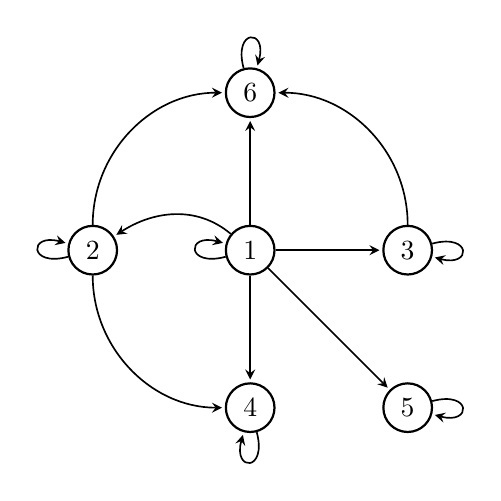
\begin{tikzpicture}[
> = stealth, % arrow head style
shorten > = 1pt, % don't touch arrow head to node
auto,
node distance = 2cm, % distance between nodes
semithick % line style
]

\tikzstyle{every state}=[
draw = black,
thick,
fill = white,
minimum size = 4mm
]

\node[state] (2) {$2$};
\node[state] (1) [right of=2] {$1$};
\node[state] (6) [above of=1] {$6$};
\node[state] (4) [below of=1] {$4$};
\node[state] (3) [right of=1] {$3$};
\node[state] (5) [below of=3] {$5$};


\path[->] (1) edge  (3);
\path[->] (1) edge  (4);
\path[->] (1) edge  (5);
\path[->] (1) edge  (6);

\draw[->] (1) to [out=140,in=33]  (2);


\draw[->] (2) to [out=270,in=180]  (4);
\draw[->] (2) to [out=90,in=180]  (6);

\draw[->] (3) to [out=90,in=0]  (6);

\draw [->] (2) edge [loop left] (2);
\draw [->] (4) edge [loop below] (4);
\draw [->] (3) edge [loop right] (3);
\draw [->] (5) edge [loop right] (5);
\draw [->] (6) edge [loop above] (6);
\draw [->] (1) edge [loop left] (1);


\end{tikzpicture}

\end{minipage}
% Creates verticle line
\hfill\vline\hfill
\begin{minipage}[t]{0.45\textwidth}
	
\subsection*{12.}
$ y\leq x $. The relation is $ \leq $.

\section*{Section 11.1}
\subsection*{14.}
Suppose $ x\in A $. Since $ R $ is symmetric, then $ xRa $ and $ aRx $, then since $ R $ is transitive then $ xRx $.

\section*{Section 11.2}
\subsection*{2.}

\[
R=
\{(a,a),(b,b),(c,c),(d,d),(e,e)
\]
\[
\newline\quad\quad,(a,d),(d,a),(b,c),(c,b),(e,d)
\]
\[
\newline,(d,e),(a,e),(e,a)
\}
\]

\end{minipage}
\pagebreak

%------------------------ End Page 1 ------------------------

%------------------------ Begin Page 2 ------------------------

\begin{minipage}[t]{0.40\textwidth}

\subsection*{10.}
\textbf{Proposition}: Suppose $ R $ and $ A $ are two equivalence relations on a set $ A $. Prove that $ R\cap S $ is also an equivalence relation.
\newline\textit{Proof.} Suppose $ (x,y)\in R\cap S $ is not an equivalence relation. Then $ (x,y)\in R $ and $ (x,y)\in S $. $ R $ and $ S $ are equivalence relations therefore  $ (x,y)\in R\cap S $ is an equivalence relation, but we said  $ (x,y)\not\in R\cap S $, a contradiction.

\subsection*{12.}
\textbf{Proposition}: Suppose $ R $ and $ S $ are equivalence relations on a set $ A $, then $ R\cup S $ is also an equivalence relation on A.
\newline\textit{Proof.} Let $ R=\{(a,a),(b,b),(c,c),(a,b),(b,a)\} $ and $ S=\{(a,a),(b,b),(c,c),(b,c),(c.b)\} $. Then $ R\cup S=$  $ \{(a,a),(b,b),(c,c),(a,b),(b,a),$  $(b,c),(c.b)\}$.
Now observe that $ (a,b)\in R \land (a,b)\in S \centernot\implies (a,b)\in R\cup S$. So $ R\cup S $ is not transitive, therefore it is not an equivalence relation.


\end{minipage}
% Creates verticle line
\hfill\vline\hfill
\begin{minipage}[t]{0.45\textwidth}

\subsection*{14.}
To show $ S $ is an equivalence relation, we must show that it's reflexive, symmetric, and transitive. To show it's reflexive, we choose an $ x\in A $ and $ n=1 $, Then $ x_1=x $ so then $ xRx $ since R is reflexive, thus $ xSx $. Now suppose $ xSy $. Then, by definition, there are elements $ x_1, x_2,...,x_n\in A$ such that $ xRx_1, x_1Rx_2,...,x_nRy $. Since $ R $ is symmetric, $ yRx_n,... x_2Rx_1, x_1Rx $, so $ ySx $. Now suppose $ xSy $ and $ ySz $. Since $ xSy $ then $ xRa, aRa_1,...a_nRy$. Since $ ySz then yRb, bRb_1,...,b_mRz $ so $ xRa,...,a_nRy,yRb1,...,b_mRz $ so $ xSz $. Now to show that $ R\subseteq S$, suppose $ (x,y)\in\mathbb{R} $. Since $ xRy, xSy $ by definition $ xSy\implies(x.y)\in S $. To show $ S $ is the smallest equivalence relation on $ A $, assume $ T $ is an equivalence relation on $ A $ containing $ R $. Suppose $ (x,y)\in S $. So $ xSy $ is $ xRx_1,...,x_nRy $ so $ xTx_1,...,x_nTy $ so $ xTx $ which shows that $ S $ is a subset of $ T $.

\section*{Section 11.3}
\subsection*{2.}
The partitions of set $ A $ are:\\
$ \{\{a\}, \{b\}, \{c\}\}, $\\
$ \{\{a,b\},\{c\}\} $,\\
$ \{\{a\},\{b,c\}\} $,\\
$ \{\{a,c\},\{b\}\} $,\\
$ \{\{a,b,c\}\} $.

\end{minipage}
\pagebreak

%------------------------ End Page 2 ------------------------

%------------------------ Begin Page 3 ------------------------

\begin{minipage}[t]{0.40\textwidth}
	
\subsection*{4.}
\textit{Proof.} Suppose $ x\in A $. Let $ X\in P $, such that $ x\in X $. Then by definition, $ xRx $. Then suppose $ xRy $ for some $ x,y\in A $, then by definition there exists a $ X\in P $ such that $ x,y\in X $. In particular, it also means $ y,x\in X $ so $ yRx $. Now suppose $ xRy $ and $ xRz $ for some $ x,y,z\in A $. Then by definition, there exists $ X_1,X_2\in P $ such that $ x,y\in X_1 $ and $ y,z\in X_2 $. Since $ P $ is a partition of $ A $, $ y $ can only be in one part, therefore $ X_1=X_2 $. Thus $ x,z\in X  \rightarrow  xRz $. Let $ X\in P $ be a part of the partition. Then by definition $ xRy $ for any two $ x,y\in X $. Also, given $ a\in X $ and $ b\in A-X $ then by definition $ a $ and $ b $ are not related. Thus $ X $ is an equivalence class of R. Since every element of $ A $ is in exactly one of the parts of $ P $, there are no equivalence classes besides the ones from the partition, thus $ P $ is the set of equivalence classes of $ R $.  
	
\section*{Section 11.4}
\subsection*{4.}

\begin{tabular}{|c|c|c|c|c|c|c|}
	\hline
	+   & [0] & [1] & [2] & [3] & [4] & [5]\\
	\hline
	[0] & [0] & [1] & [2] & [3] & [4] & [5]\\
	\hline
	[1] & [1] & [2] & [3] & [4] & [5] & [0]\\
	\hline
	[2] & [2] & [3] & [4] & [5] & [0] & [1]\\
	\hline
	[3] & [3] & [4] & [5] & [0] & [1] & [2]\\
	\hline
	[4] & [4] & [5] & [0] & [1] & [2] & [3]\\
	\hline
	[5] & [5] & [0] & [1] & [2] & [3] & [4]\\
	\hline
\end{tabular}

\begin{tabular}{|c|c|c|c|c|c|c|}
	\hline
	$ \cdot $   & [0] & [1] & [2] & [3] & [4] & [5]\\
	\hline
	[0] & [0] & [0] & [0] & [0] & [0] & [0]\\
	\hline
	[1] & [0] & [1] & [2] & [3] & [4] & [5]\\
	\hline
	[2] & [0] & [2] & [4] & [0] & [2] & [4]\\
	\hline
	[3] & [0] & [3] & [0] & [3] & [0] & [3]\\
	\hline
	[4] & [0] & [4] & [2] & [0] & [4] & [2]\\
	\hline
	[5] & [0] & [5] & [4] & [3] & [2] & [1]\\
	\hline
\end{tabular}

\end{minipage}
% Creates verticle line
\hfill\vline\hfill
\begin{minipage}[t]{0.45\textwidth}
	
\subsection*{6.}
No, because in $ \mathbb{Z}_6 $, for example, $ [a] $ could be $ [3] $ and $ [b] $ could be $ [4] $ which would be $ [4]\cdot[3]=[12]=[0] $. As long as $ [a]\cdot[b] $ results in a multiple of $ 6 $ then the result will be $ [0] $.


\subsection*{8.} By definition, $ [a]=[a'] $ is $ a\equiv a'\pmod n $ so $ n|a-a' \rightarrow a-a'=nk, k\in\mathbb{Z}$. Similarly, $ [b]=[b'] $ is  $ b\equiv b'\pmod n $ so $ n|b-b' \rightarrow b-b'=nm, m\in\mathbb{Z}$. Then we can say $ a=a'+nk $ and $ b=b'+nm $. If we add them together, we get $ a+b=(a'+b')+nk+nm \rightarrow (a+b)-(a'+b')=n(k+m)\rightarrow (a+b)-(a'+b')=nh, h=(k+m)\in\mathbb{Z}$. Therefore $ n|(a+b)-(a'+b')\rightarrow (a+b)\equiv(a'+b')\pmod n $. Therefore in $ \mathbb{Z}_n $, $ [a+b]=[a'+b'] $.
	
	

\end{minipage}
\pagebreak

%------------------------ End Page 4 ------------------------

\end{document}
